\documentclass[11pt]{article}
\usepackage[margin=2.2cm]{geometry}
\usepackage{graphicx}
\usepackage{float}
\usepackage{xcolor}
\usepackage{framed}
\usepackage[hidelinks]{hyperref}
\setlength{\parskip}{6pt}
\setlength{\parindent}{0pt}
\definecolor{quotebg}{RGB}{247,247,247}
\newenvironment{proposalquote}{\begin{leftbar}\small\itshape}{\end{leftbar}}

\title{LFS, from the proposal to the ruler\\[4pt]\large A plain-language study document, one idea per picture}
\author{Waiz Khan}
\date{10 September 2026}

\begin{document}
\maketitle

\section*{How to read this}
Read it in order. Each picture carries one idea, and the paragraph under it says the idea in the simplest words I have. Part A is what the NSF proposal asks in Aim 1. Part B is how we answered it. Part C is how the ruler works, step by step, with arithmetic you can do by hand. Part D is what to say back from memory. Every number is from a stored result; nothing is rounded to look nicer.

\section*{Part A. What Aim 1 of the proposal asks}

\subsection*{A.1 The worry}
\begin{figure}[H]\centering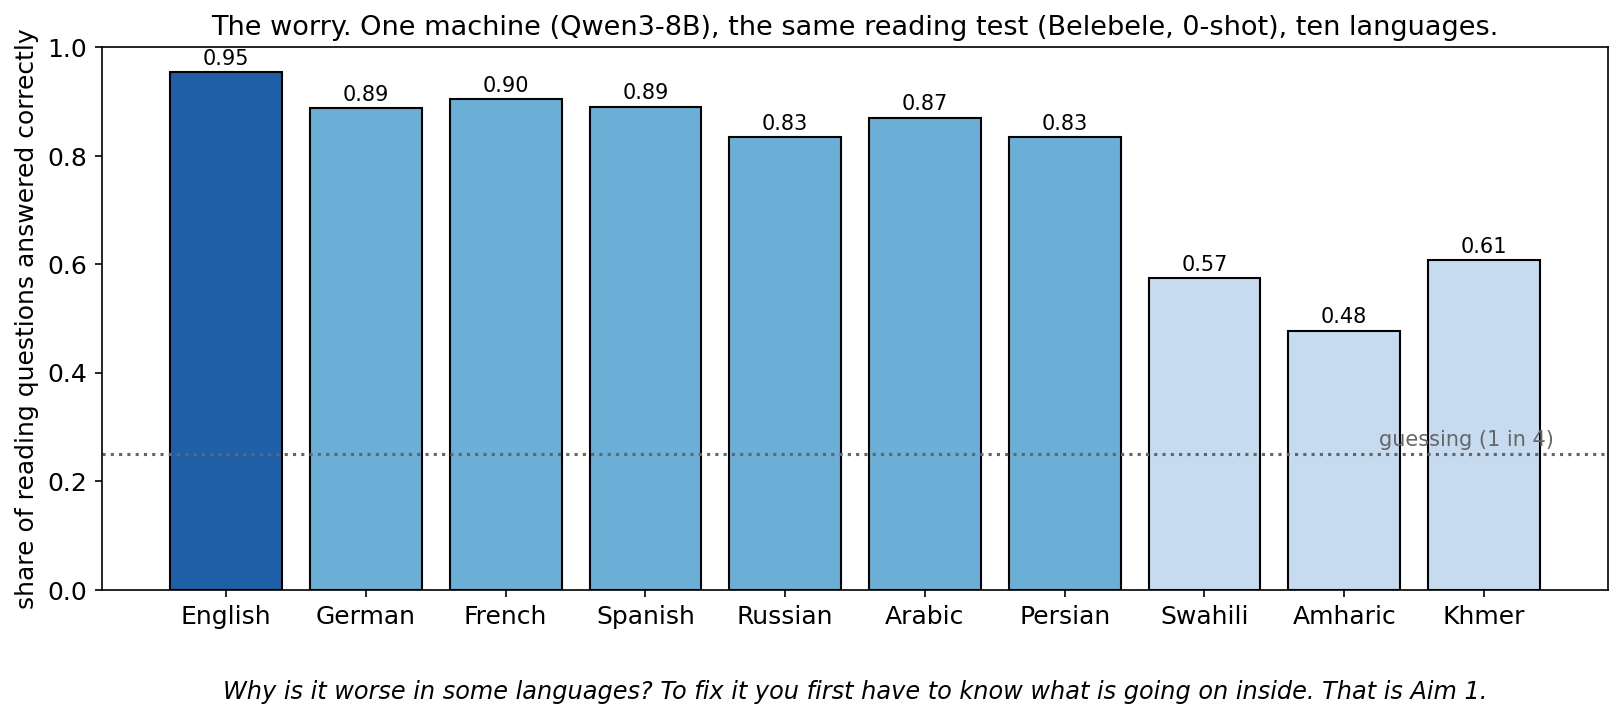
\includegraphics[width=0.95\linewidth]{figs/proposal/p1_worry.png}\end{figure}
A machine read most of the books in the world, and most of those books were in English. Give it the same reading test in ten languages and it does best in English and worst in Amharic. The professors want to make the machine equally good in every language. But you cannot fix a machine you cannot see into. So before fixing, Aim 1 says: look inside and understand.

The proposal states the goal in one sentence:
\begin{proposalquote}
``\ldots how large language models handle different languages, especially how the same concepts are represented when presented in different languages, and how they can access information across languages.''
\end{proposalquote}

\subsection*{A.2 The proposal's picture of the machine}
\begin{figure}[H]\centering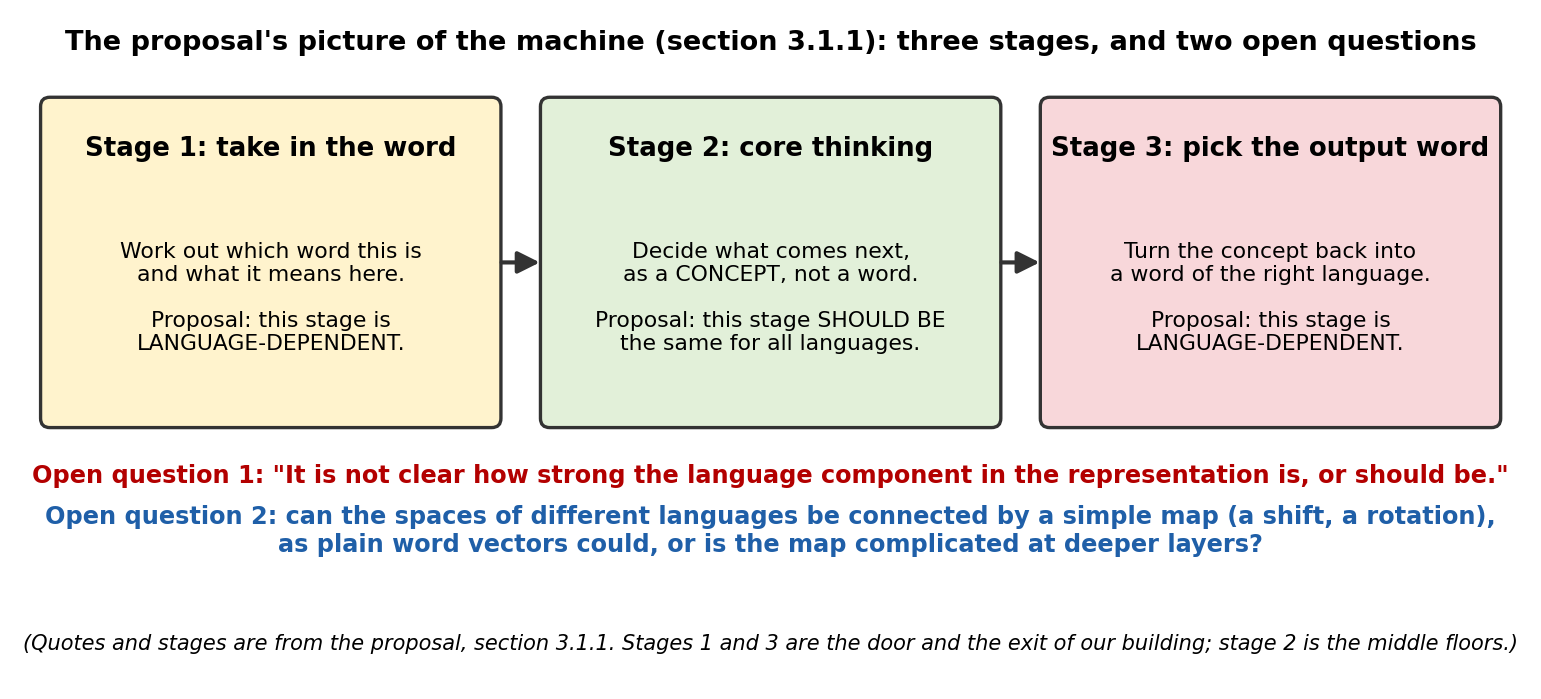
\includegraphics[width=0.98\linewidth]{figs/proposal/p2_three_stages.png}\end{figure}
Section 3.1.1 of the proposal says the machine works in three stages. Stage 1 takes in the new word. Stage 2 does the core thinking, about the concept, not the word. Stage 3 picks the output word. The professors expect stages 1 and 3 to depend on the language, and they argue stage 2 should be the same for every language. Then they say, in their own words, what nobody knows:
\begin{proposalquote}
``It is not clear how strong the language component in the representation is, or should be in models that would be more robust across languages.''
\end{proposalquote}
That sentence is the seed of LFS. LFS is a number that says exactly how strong the language component is, at every stage.

\subsection*{A.3 The four tasks}
\begin{figure}[H]\centering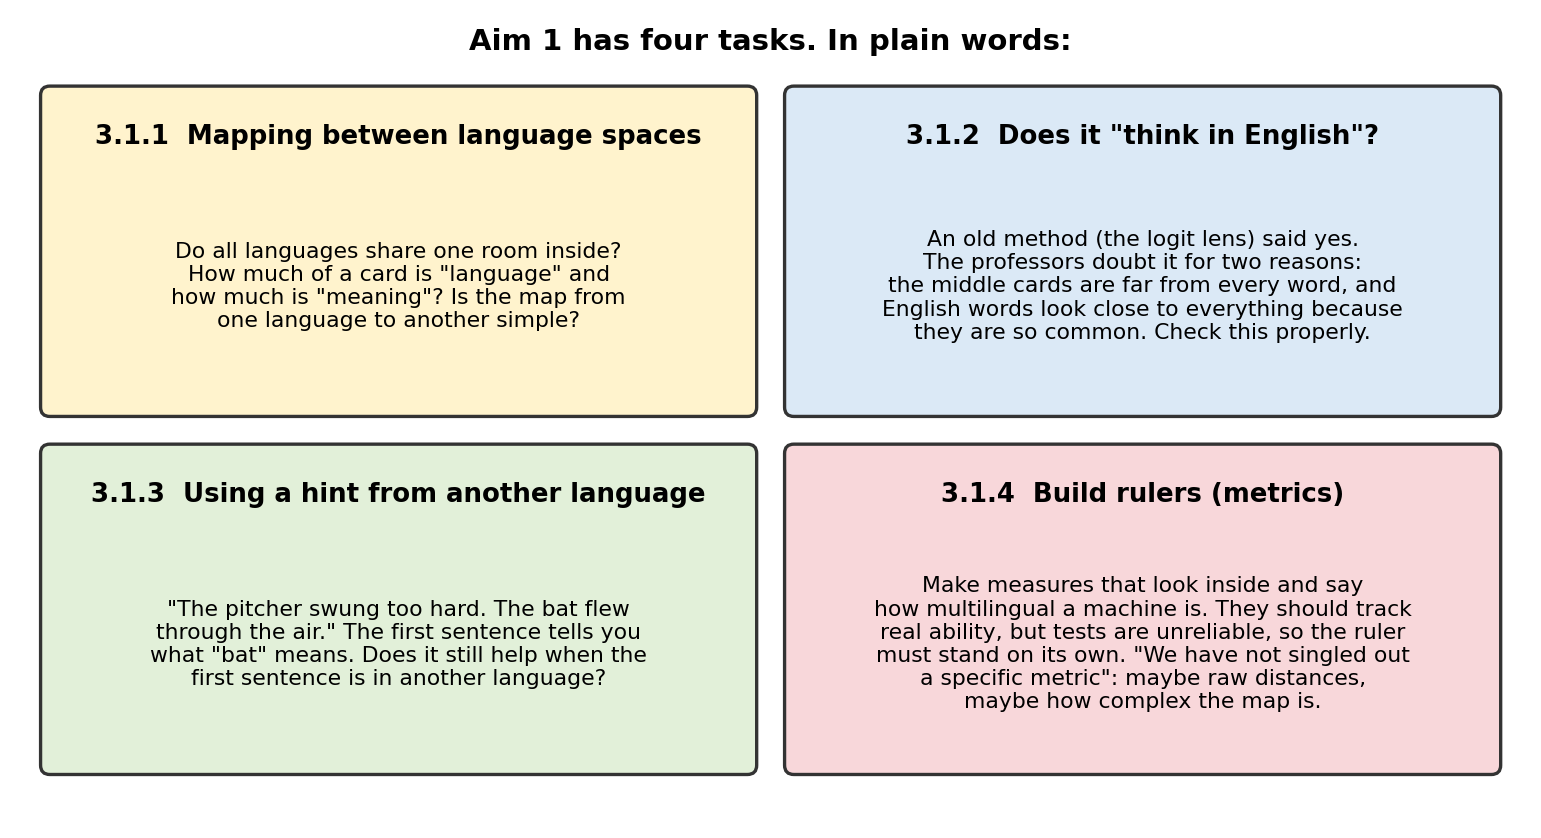
\includegraphics[width=0.98\linewidth]{figs/proposal/p3_four_tasks.png}\end{figure}
Task 3.1.1 asks whether the language spaces can be mapped onto each other with a simple map, and what that map says about which parts of a card carry knowledge and which carry language. Task 3.1.2 revisits the claim that machines ``think in English''; the professors give two reasons to doubt it. Task 3.1.3 asks whether a hint given in another language still helps the machine understand a later sentence. Task 3.1.4 asks for rulers:
\begin{proposalquote}
``\ldots we will develop intrinsic metrics to measure the similarity of representation spaces that will serve as immediate feedback for research and may even be used directly as a training objective. \ldots At this point, we have not singled out a specific metric.''
\end{proposalquote}

\subsection*{A.4 What a ruler must be able to answer}
\begin{figure}[H]\centering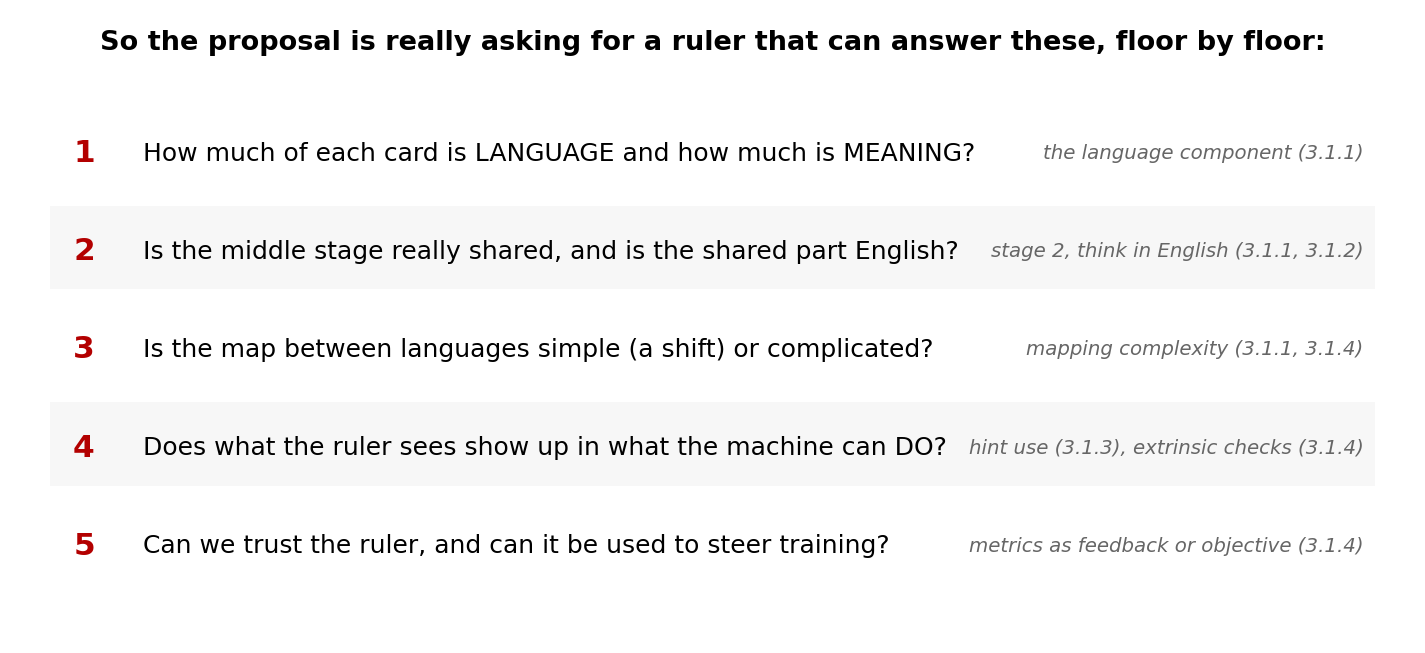
\includegraphics[width=0.95\linewidth]{figs/proposal/p4_wishlist.png}\end{figure}
Put the four tasks together and the proposal is asking for a ruler that can answer five questions, floor by floor: how much is language and how much is meaning; is the middle really shared and is it English; is the map simple; does any of this show in what the machine can do; and can the ruler be trusted, or even used to steer training.

\section*{Part B. How we answered it}

\subsection*{B.1 The two possible pictures}
\begin{figure}[H]\centering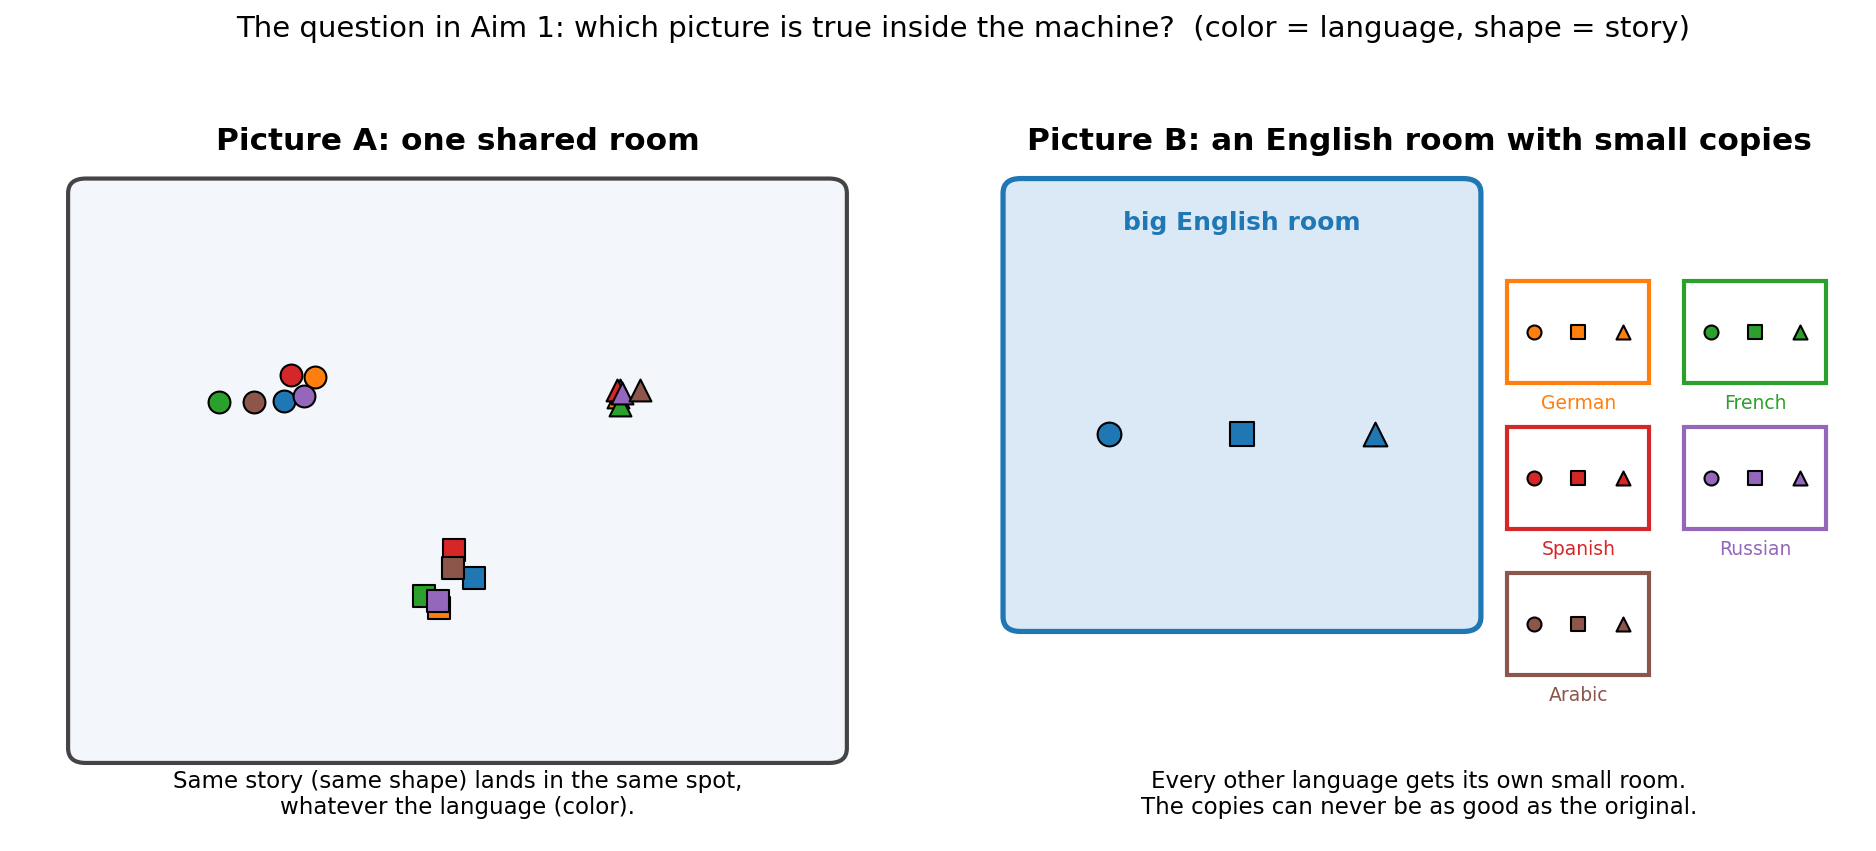
\includegraphics[width=0.98\linewidth]{figs/story/story1_problem.png}\end{figure}
Before measuring, say what the two answers would look like. Picture A: one shared room where the same story lands in the same spot whatever the language. Picture B: a big English room with a small copy for every other language. The proposal's three-stage picture is a bet on A for the middle stage. Our job was to find out.

\subsection*{B.2 The ruler in four steps}
\begin{figure}[H]\centering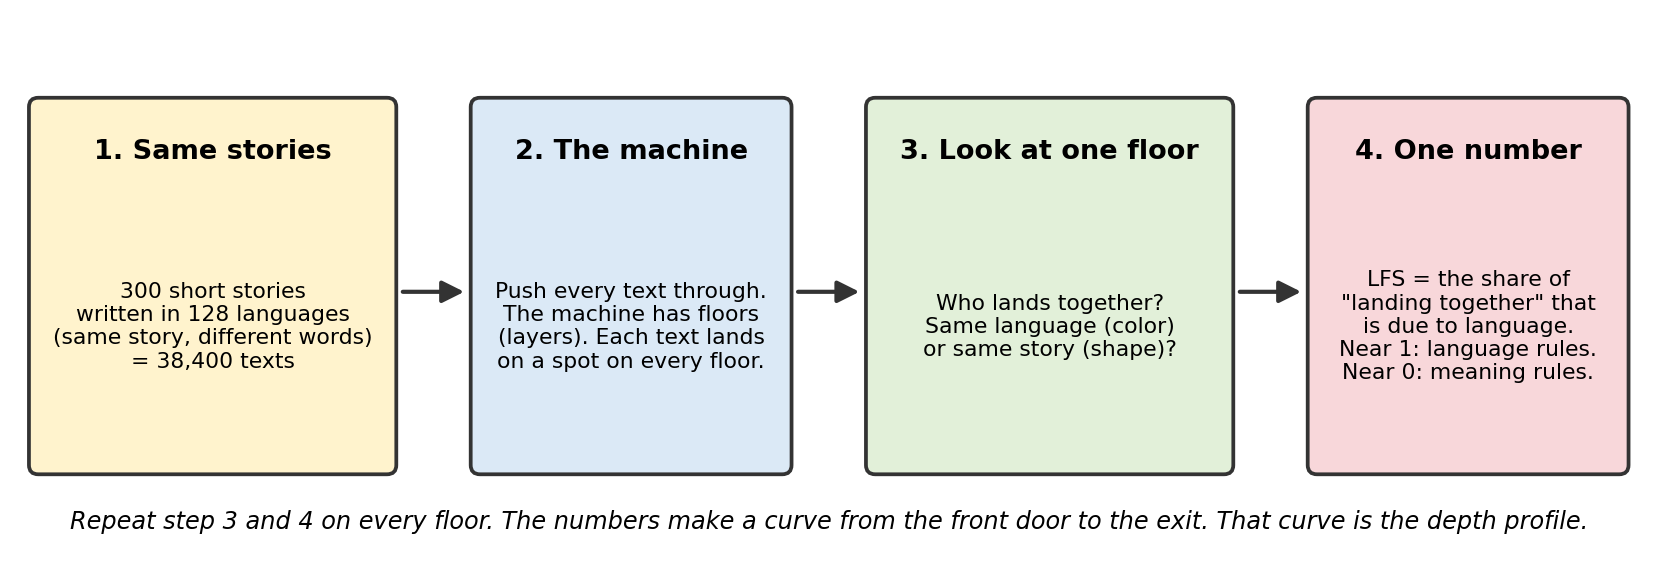
\includegraphics[width=0.98\linewidth]{figs/story/story2_ruler.png}\end{figure}
Take the same 300 stories in 128 languages. Push every text through the machine. On each floor, ask who lands together: same language, or same story? LFS is the share of ``landing together'' that is due to language. Do it on every floor and you get a curve. Part C shows the arithmetic.

\subsection*{B.3 One measure per question}
\begin{figure}[H]\centering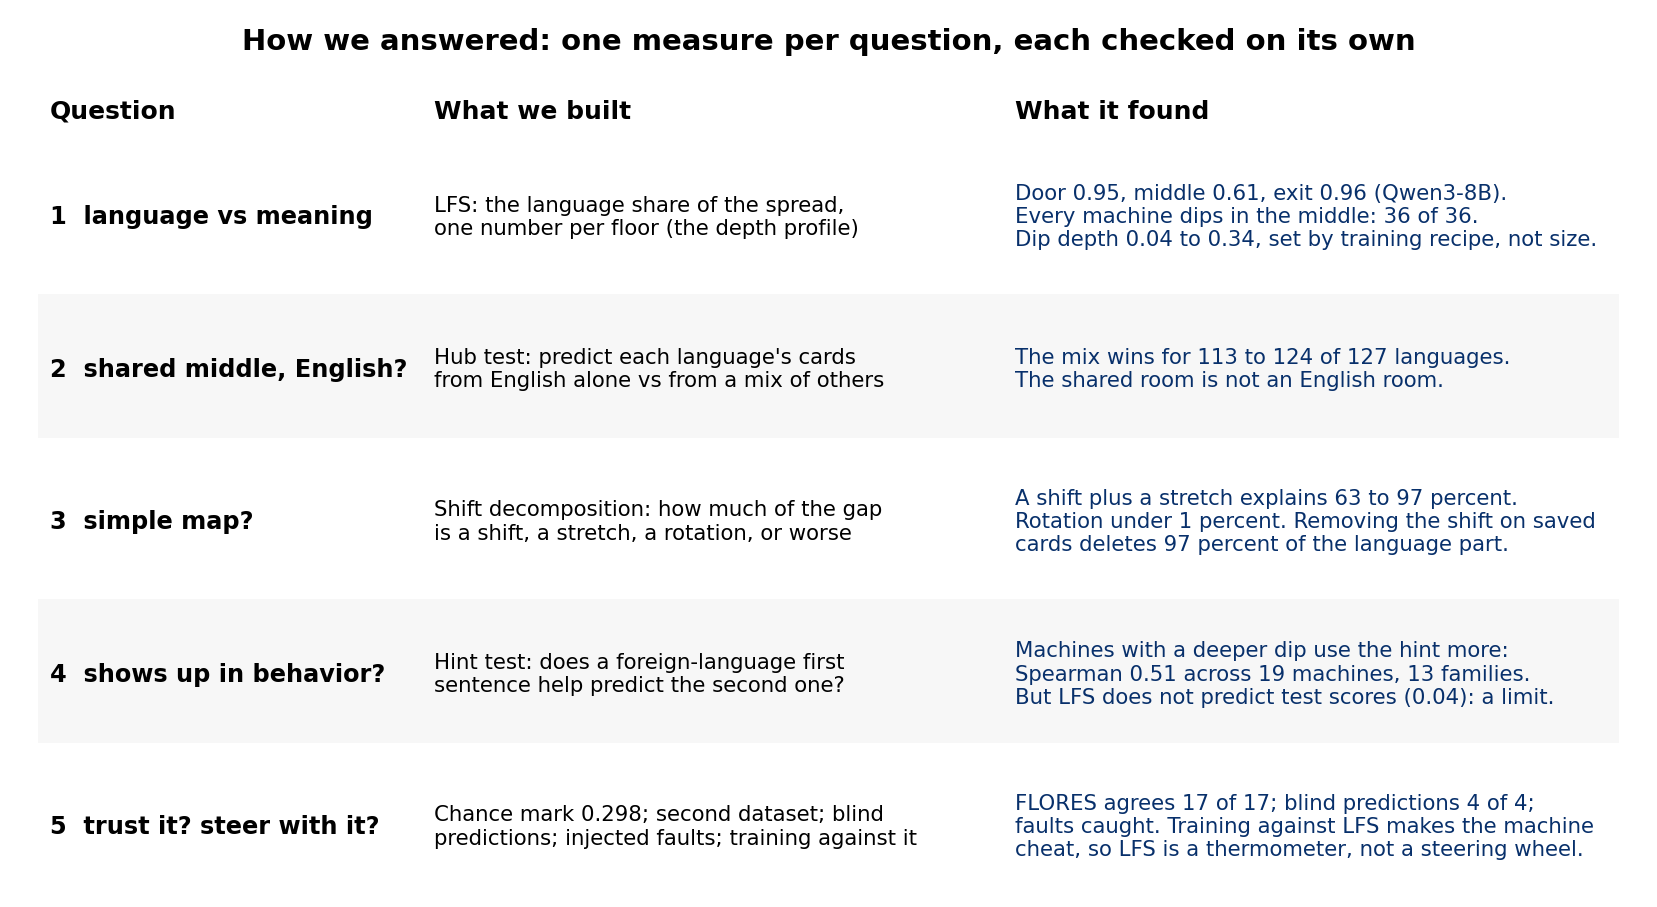
\includegraphics[width=0.98\linewidth]{figs/proposal/b1_answers_table.png}\end{figure}
We did not build one number and call it done. Each of the five questions got its own measure, and each measure was checked on its own question. The LFS curve answers question 1. The hub test answers question 2. The shift decomposition answers question 3. The hint test answers question 4. The chance mark, a second dataset, blind predictions, injected faults, and a training experiment answer question 5. The proposal asked for metrics, plural, and this is the plural.

\subsection*{B.4 The verdict}
\begin{figure}[H]\centering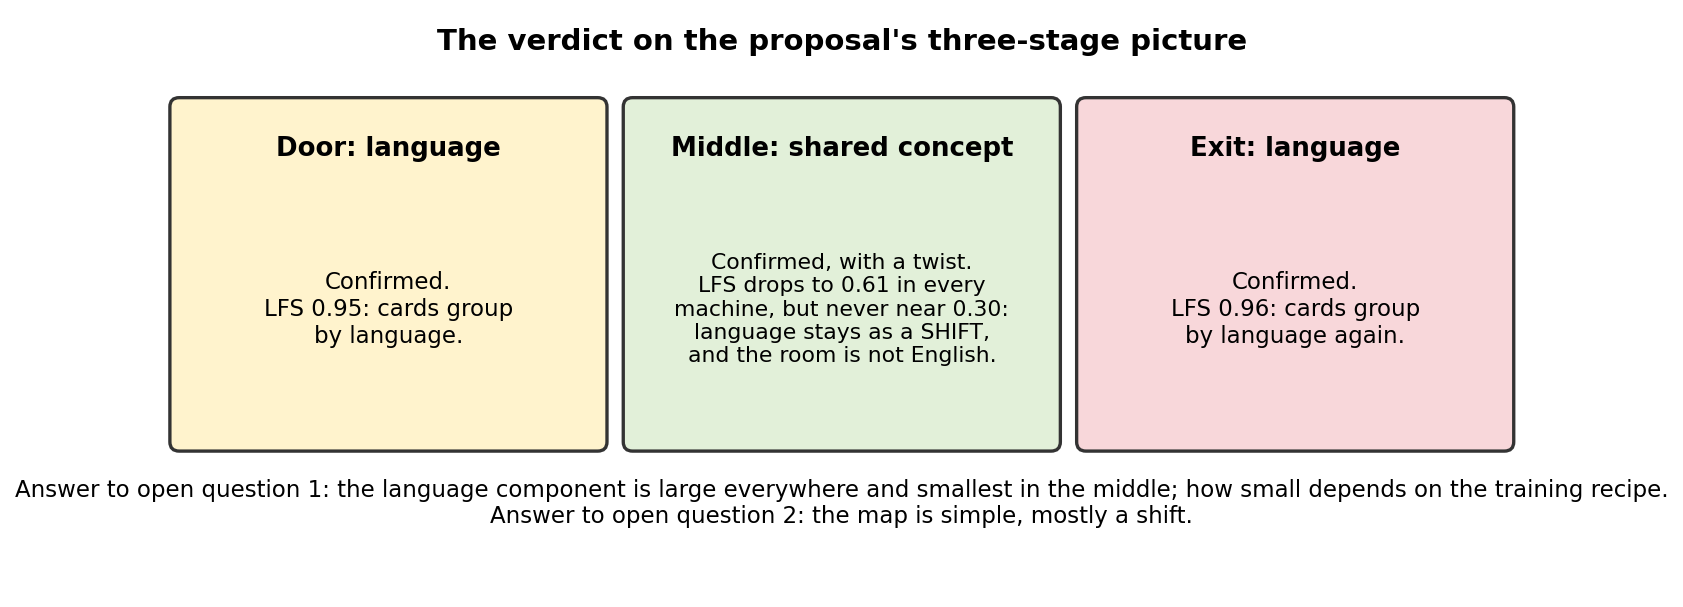
\includegraphics[width=0.98\linewidth]{figs/proposal/b2_verdict.png}\end{figure}
\begin{figure}[H]\centering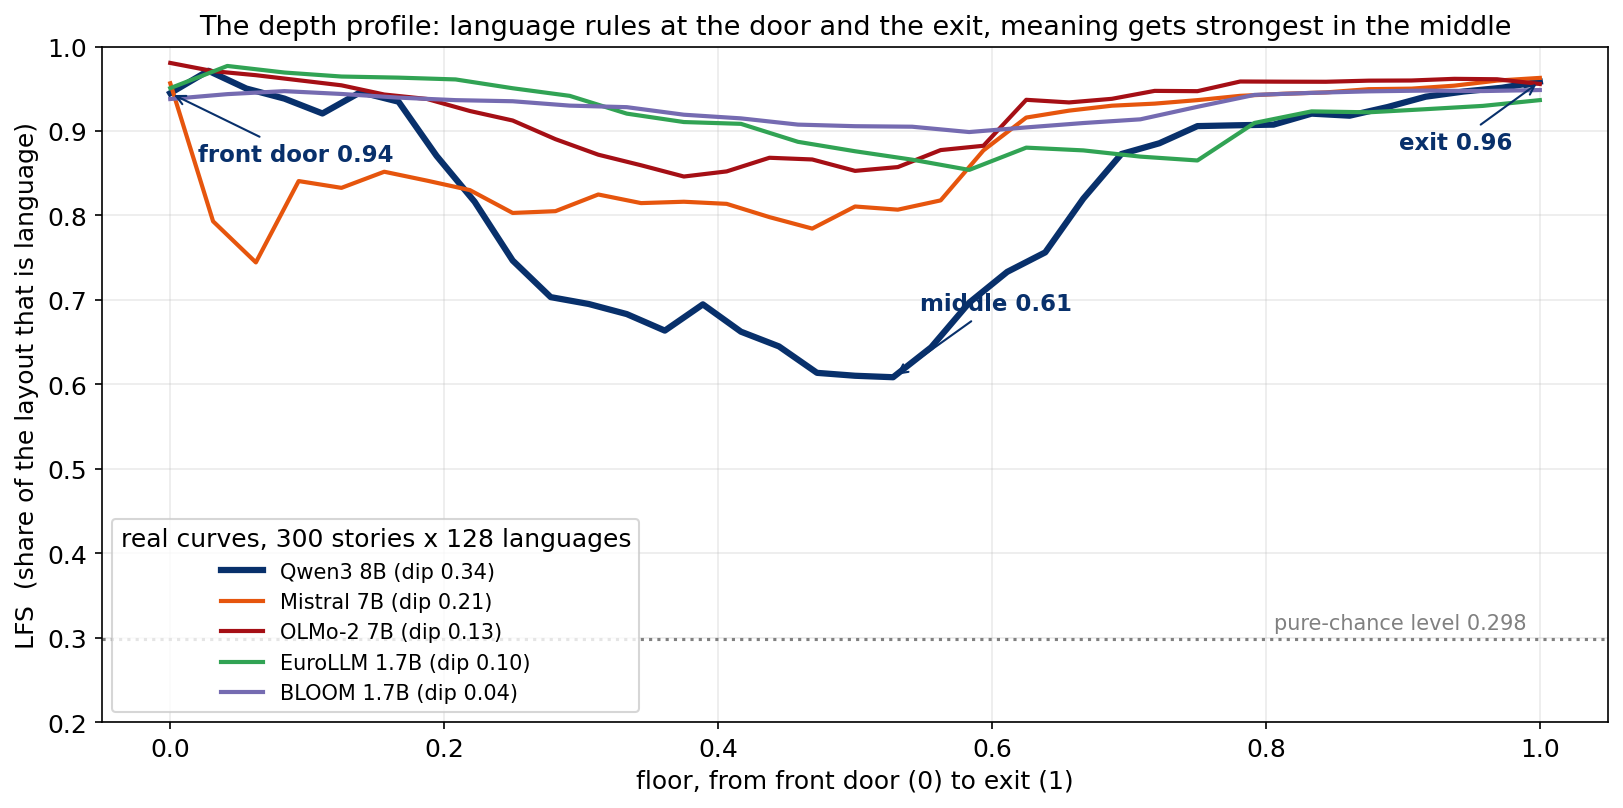
\includegraphics[width=0.9\linewidth]{figs/story/story4_curve.png}\end{figure}
The three-stage picture holds, with one twist. Language rules at the door and at the exit. In the middle the same story lands close in every language, in every one of the 36 machines we measured. But the language component never goes away; it stays as a shift, and how small it gets depends on how the machine was taught, not on how big it is.
\begin{figure}[H]\centering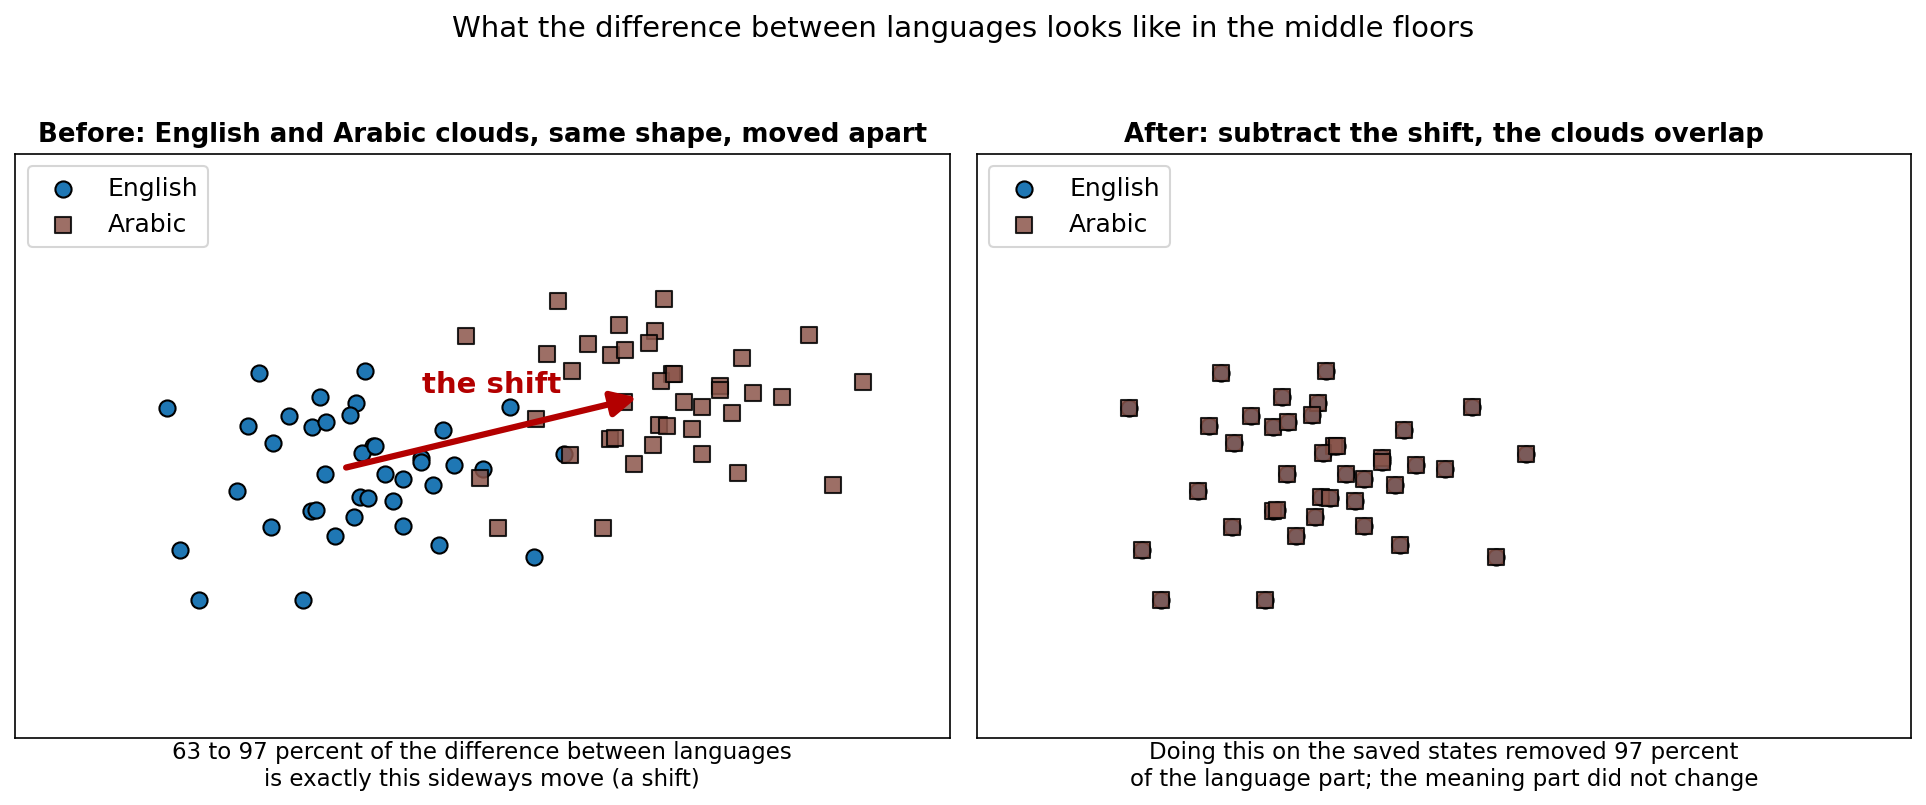
\includegraphics[width=0.98\linewidth]{figs/story/story5_shift.png}\end{figure}
The shift is the answer to the mapping question: the map between languages is simple. Subtract each language's shift and the clouds overlap. On the saved cards, that single move removes 97 percent of the language part and leaves the meaning part untouched.

\section*{Part C. How the ruler works, step by step}
Twelve steps. Steps 1 to 4 are about getting the cards into a table. Steps 5 to 7 are the arithmetic on a tiny pretend table you can do by hand. Steps 8 to 10 scale it up to the real thing. Steps 11 and 12 are the limits and the link back to the proposal.

\subsection*{Step 1. Words become cards}
\begin{figure}[H]\centering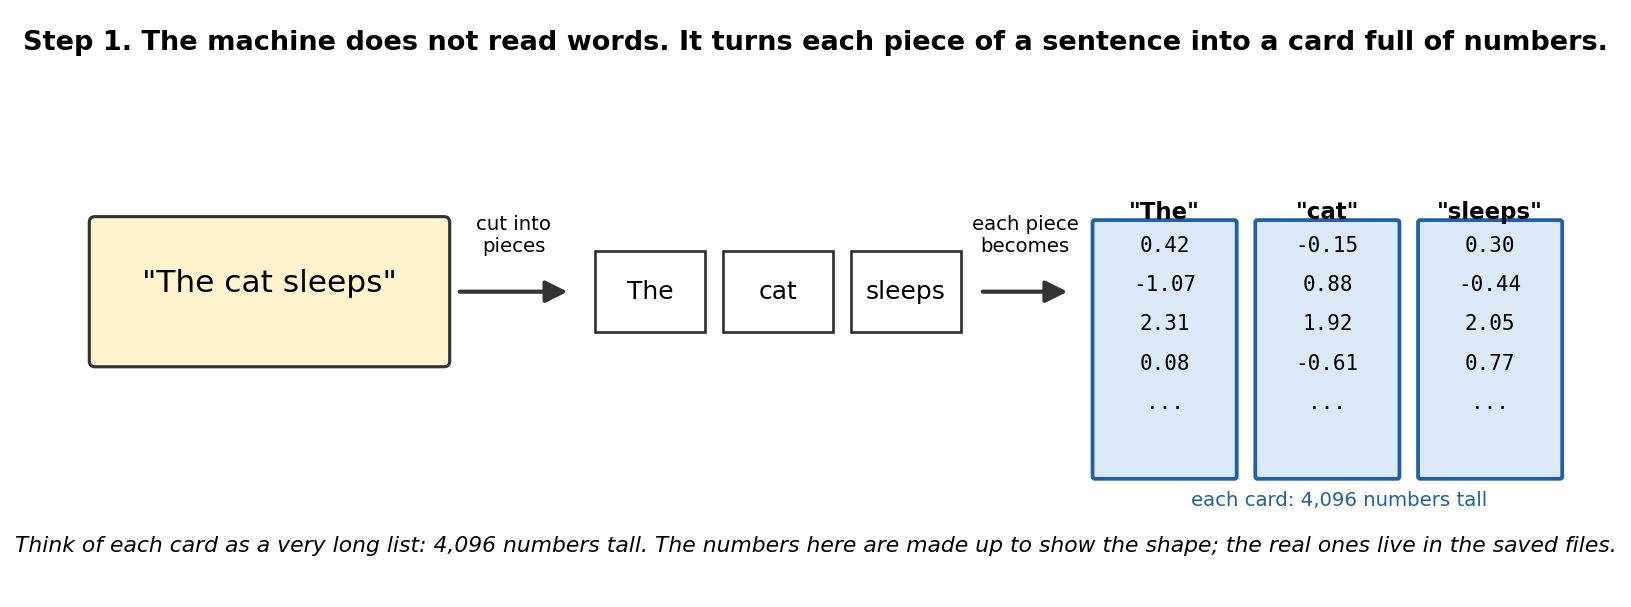
\includegraphics[width=0.98\linewidth]{figs/steps/s01_sentence_to_cards.png}\end{figure}
The machine cannot read. It cuts a sentence into pieces and turns each piece into a card with 4,096 numbers on it. A card is just a very long list of numbers.

\subsection*{Step 2. Floors}
\begin{figure}[H]\centering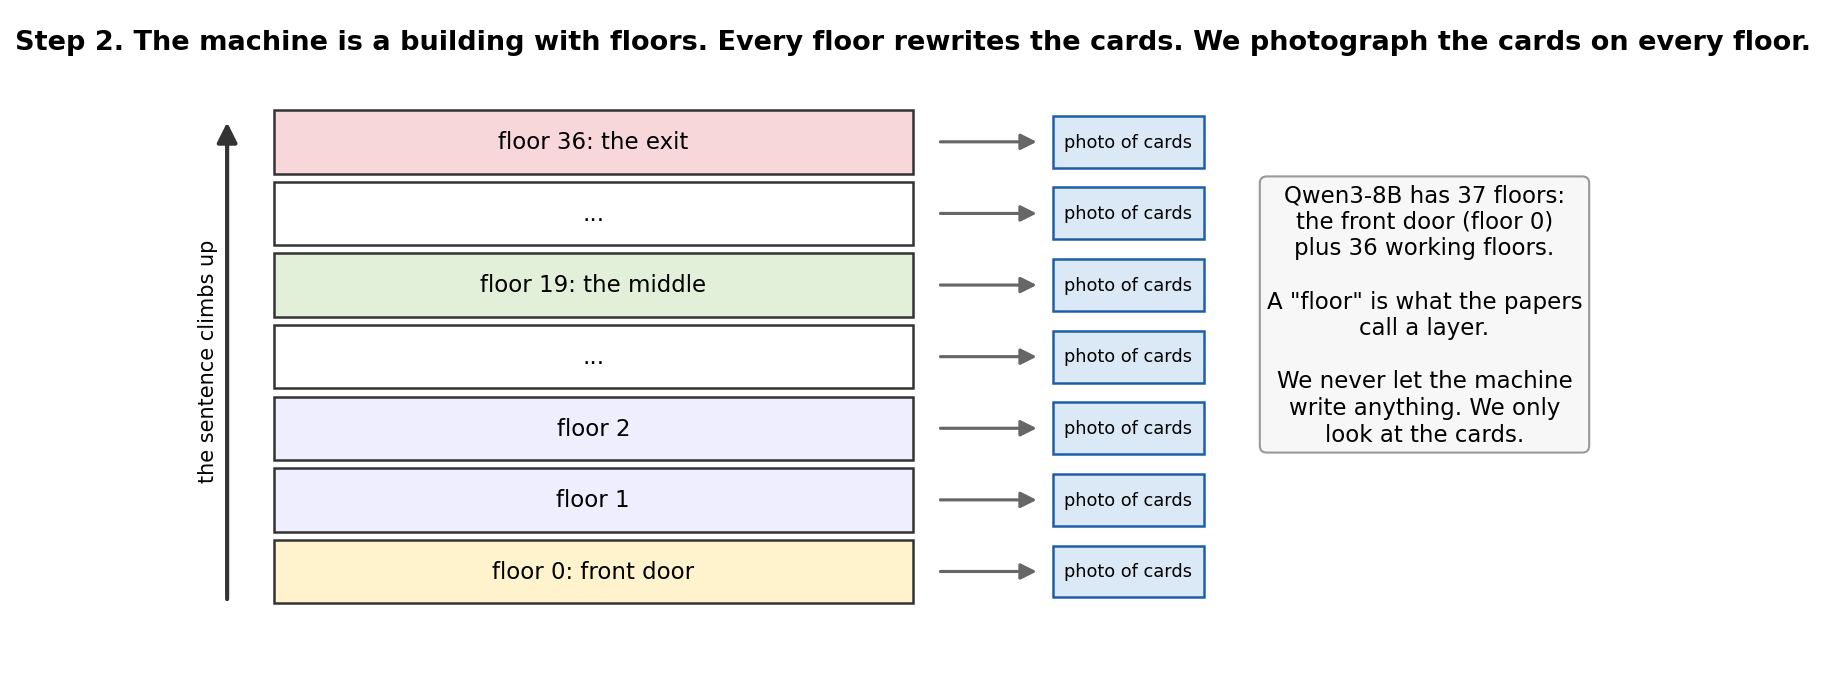
\includegraphics[width=0.98\linewidth]{figs/steps/s02_floors.png}\end{figure}
The machine is a building. Cards go in at the front door and climb up. Every floor rewrites the numbers a little. Qwen3-8B has 36 working floors above the door. We photograph the cards on every floor. We never let the machine talk.

\subsection*{Step 3. Averaging}
\begin{figure}[H]\centering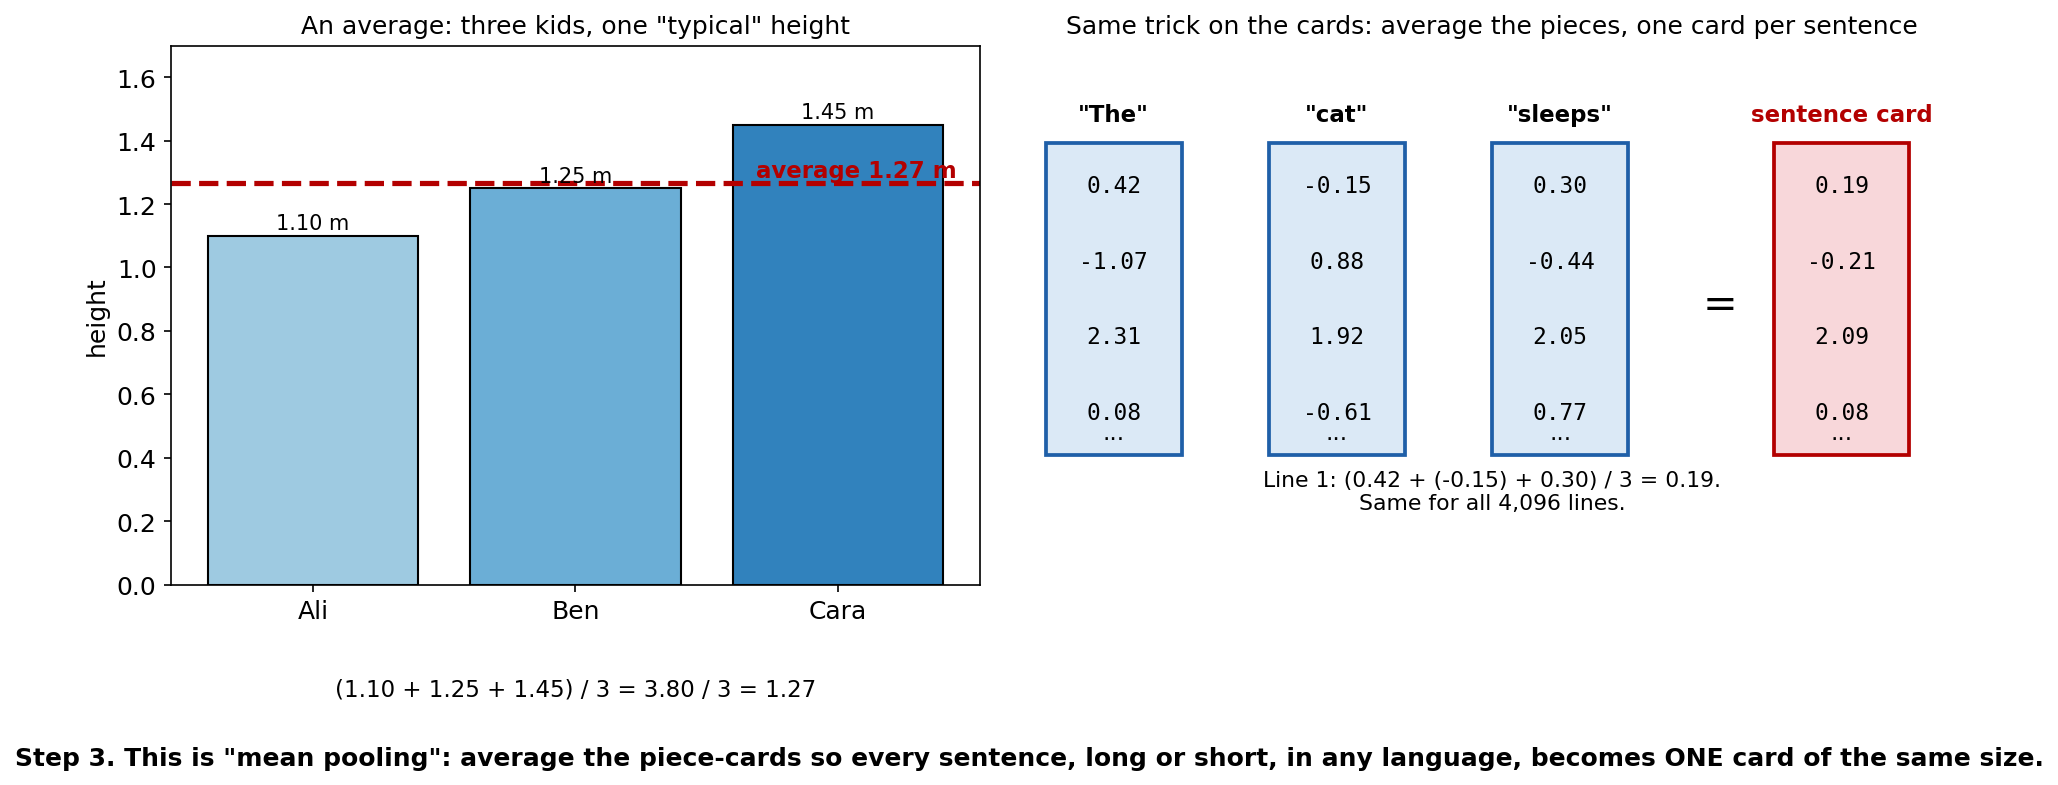
\includegraphics[width=0.98\linewidth]{figs/steps/s03_mean_pooling.png}\end{figure}
Three kids are 1.10, 1.25, and 1.45 meters tall. Add: 3.80. Divide by three: 1.27. That is the typical height. Do the same to the piece-cards, line by line, and you get one card per sentence. Every sentence, short or long, in any language, becomes one card of the same size. That is all ``mean pooling'' means.

\subsection*{Step 4. The table}
\begin{figure}[H]\centering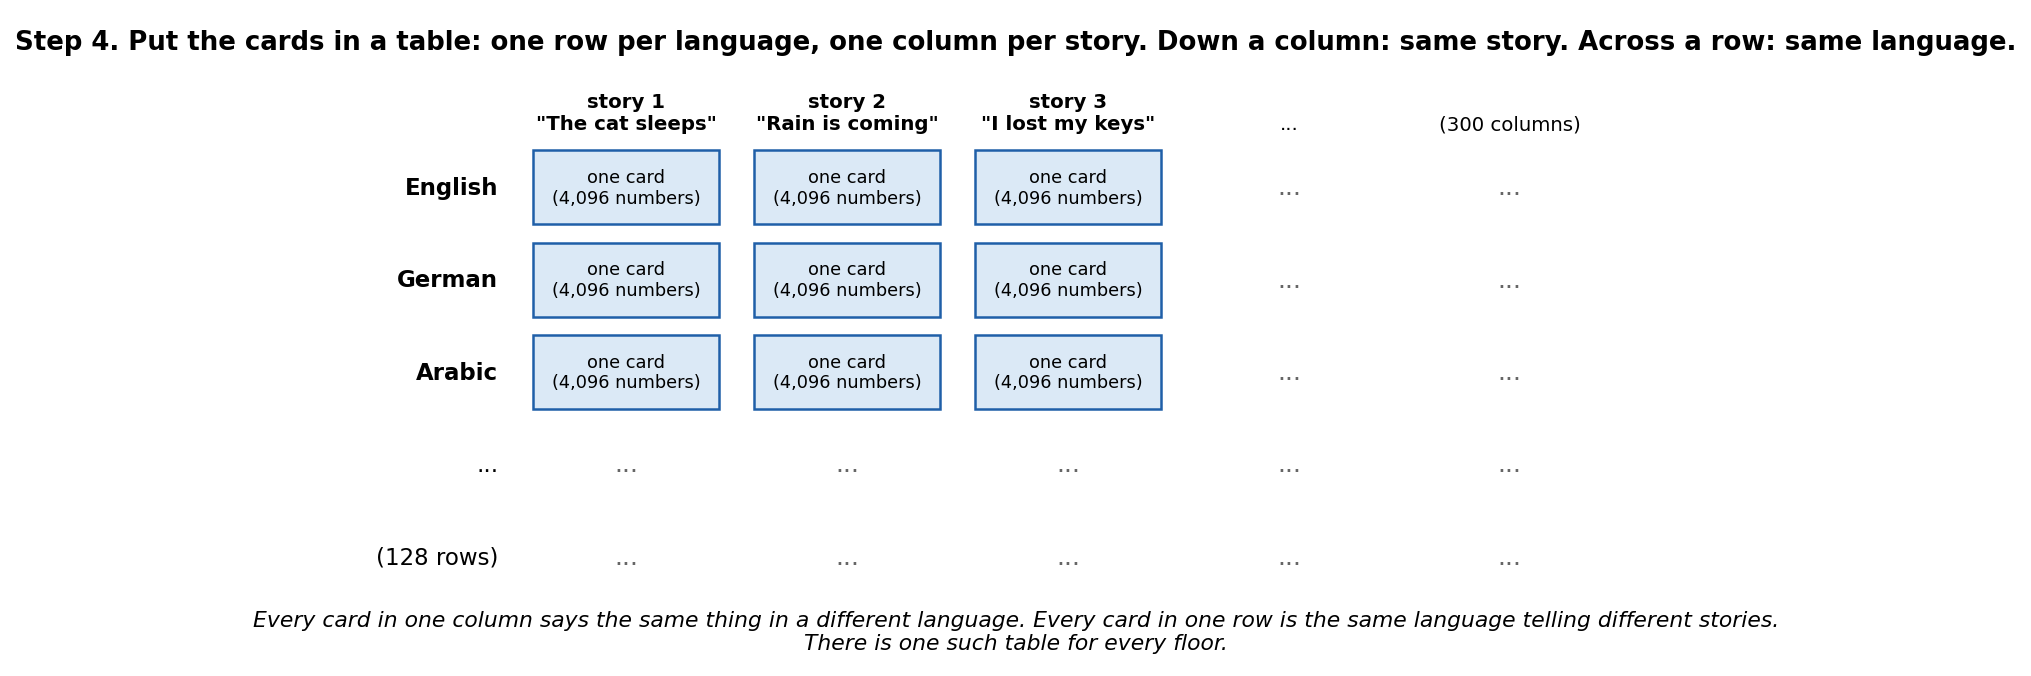
\includegraphics[width=0.98\linewidth]{figs/steps/s04_table.png}\end{figure}
Languages go down, stories go across, one card in each box. Down a column is the same story in different languages. Across a row is the same language telling different stories. Every floor has its own table.

\subsection*{Step 5. A tiny pretend table}
\begin{figure}[H]\centering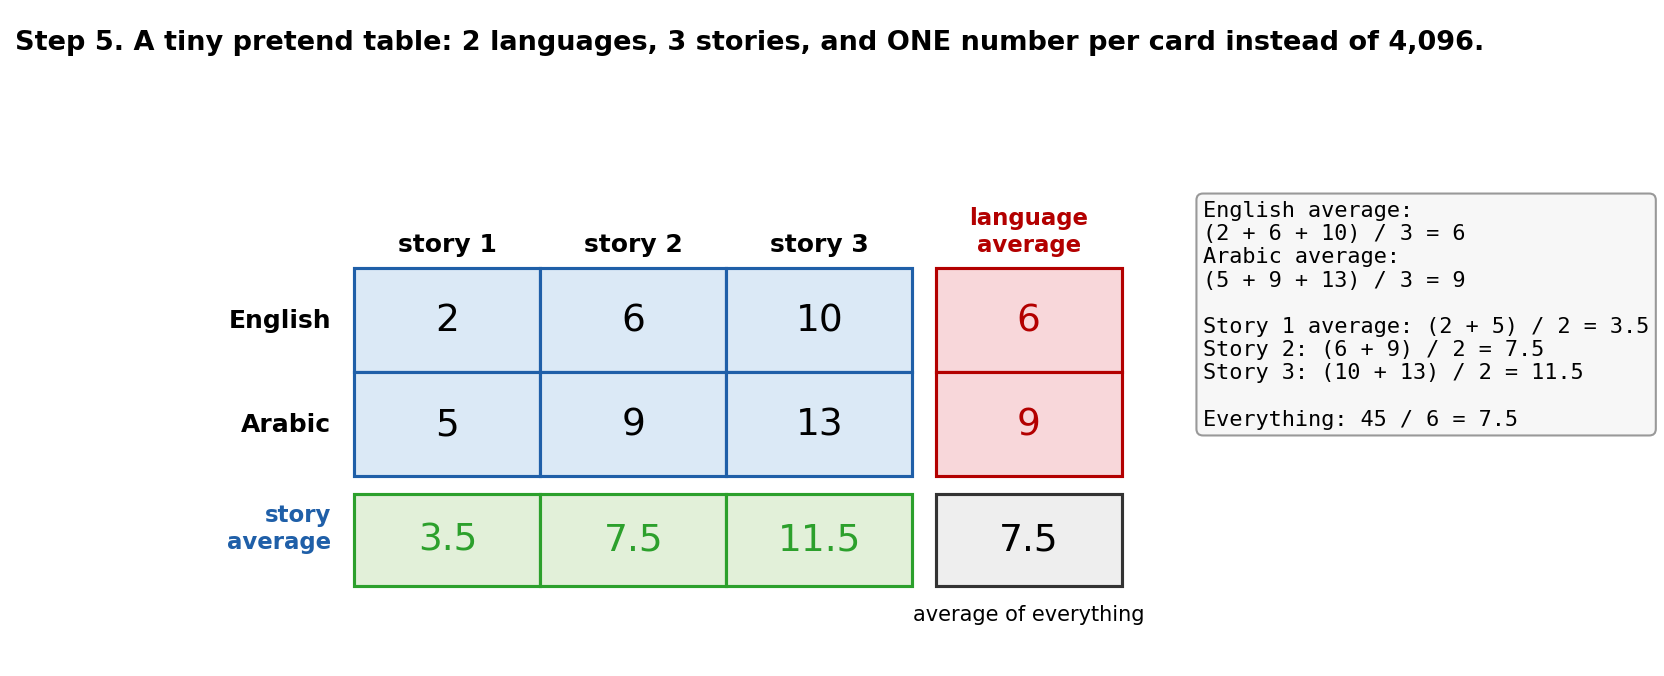
\includegraphics[width=0.95\linewidth]{figs/steps/s05_tiny_table.png}\end{figure}
Pretend a card has one number, and there are two languages and three stories. English: 2, 6, 10. Arabic: 5, 9, 13. English average 6, Arabic average 9. Story averages 3.5, 7.5, 11.5. Average of everything 7.5.

\subsection*{Step 6. Spread, drawn as squares}
\begin{figure}[H]\centering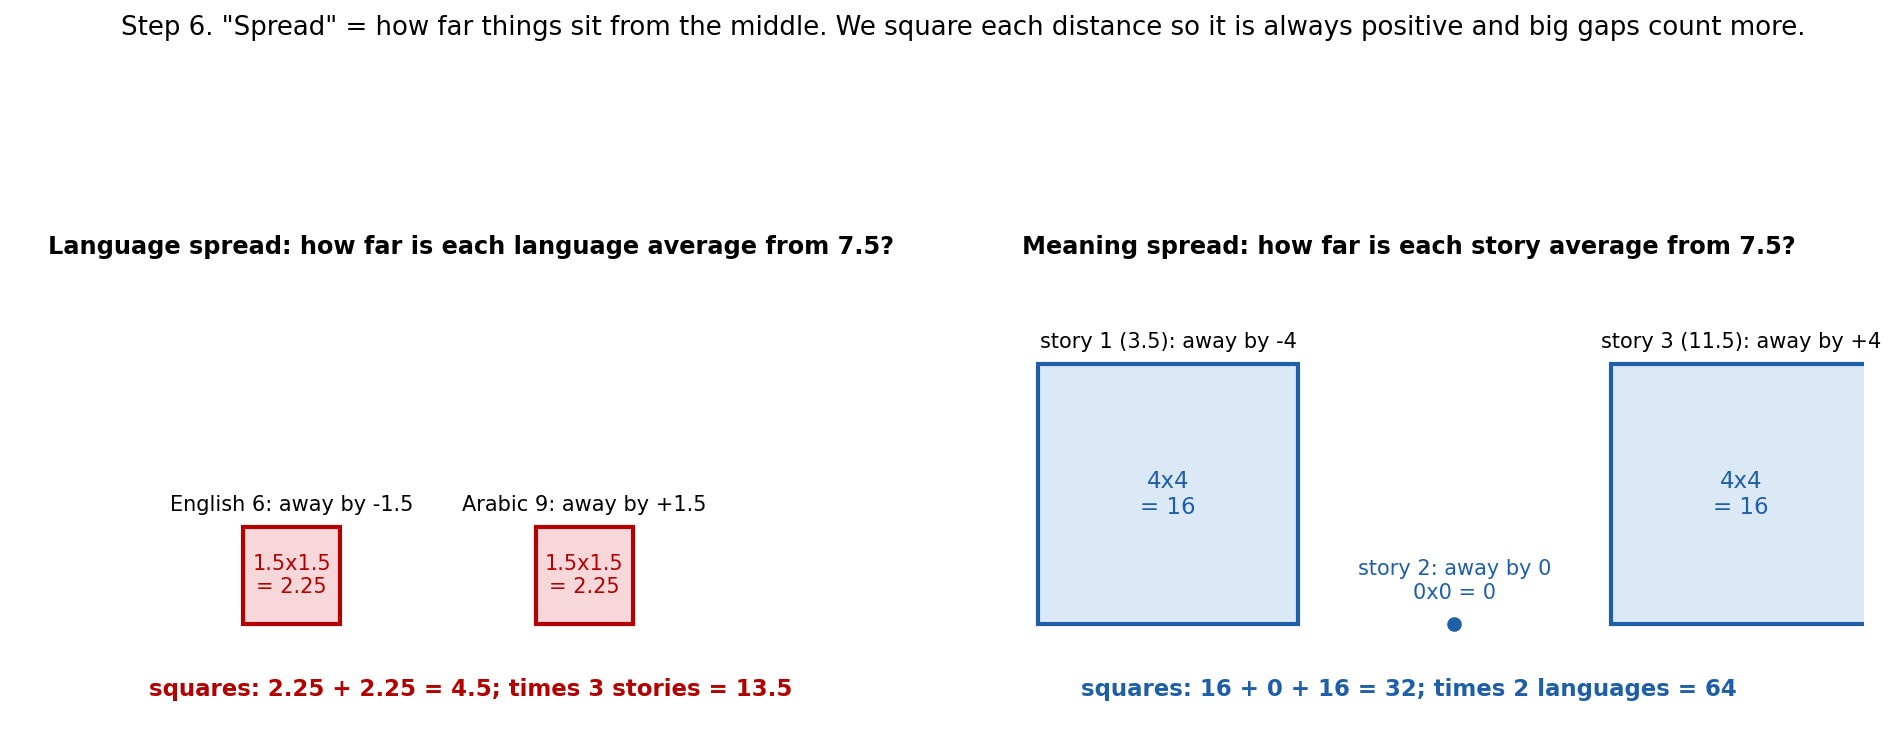
\includegraphics[width=0.98\linewidth]{figs/steps/s06_spread_squares.png}\end{figure}
Spread means how far things sit from the middle. English is 1.5 below 7.5 and Arabic is 1.5 above. A square with side 1.5 has area 2.25; two of them make 4.5; each language average stands for three stories, so times three: 13.5. That is the language spread. Story 1 is 4 below, story 3 is 4 above, story 2 is on the middle: squares of area 16, 16, and 0 make 32; each story average stands for two languages, so times two: 64. That is the meaning spread. We use squares so that below and above do not cancel, and so big gaps count more.

\subsection*{Step 7. The share}
\begin{figure}[H]\centering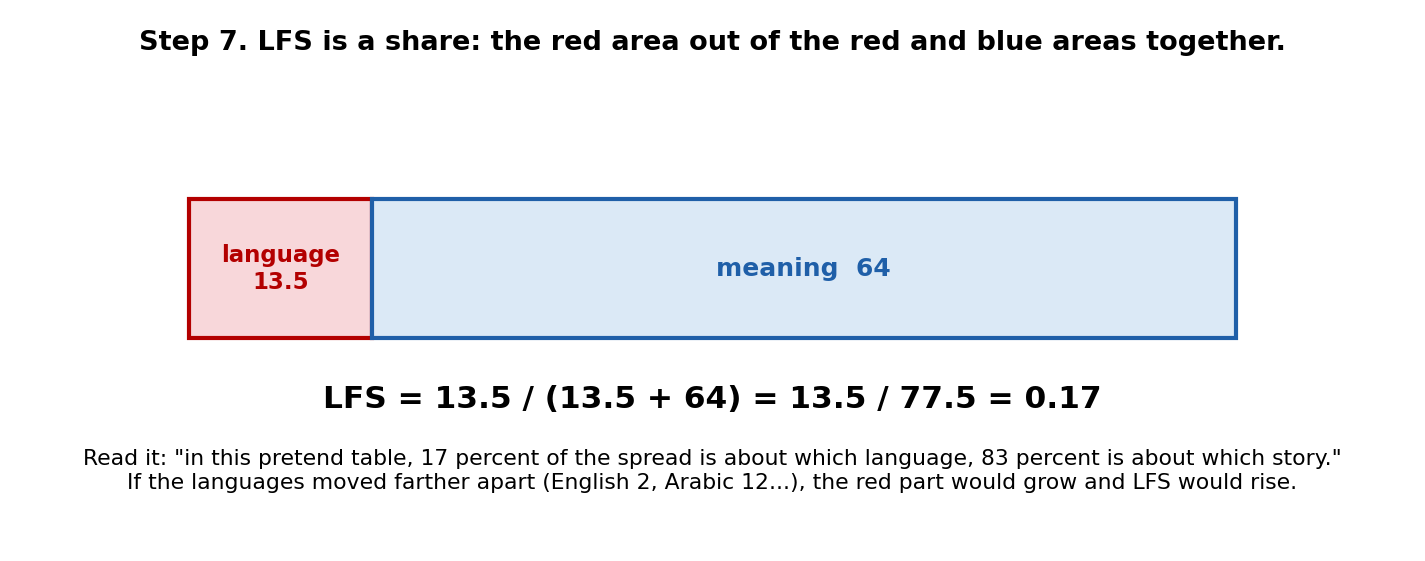
\includegraphics[width=0.9\linewidth]{figs/steps/s07_share.png}\end{figure}
LFS is the red part out of the whole bar: 13.5 out of 77.5, which is 0.17. Say it in words: 17 percent of the spread is about which language, 83 percent is about which story.

\subsection*{Step 8. Real cards}
\begin{figure}[H]\centering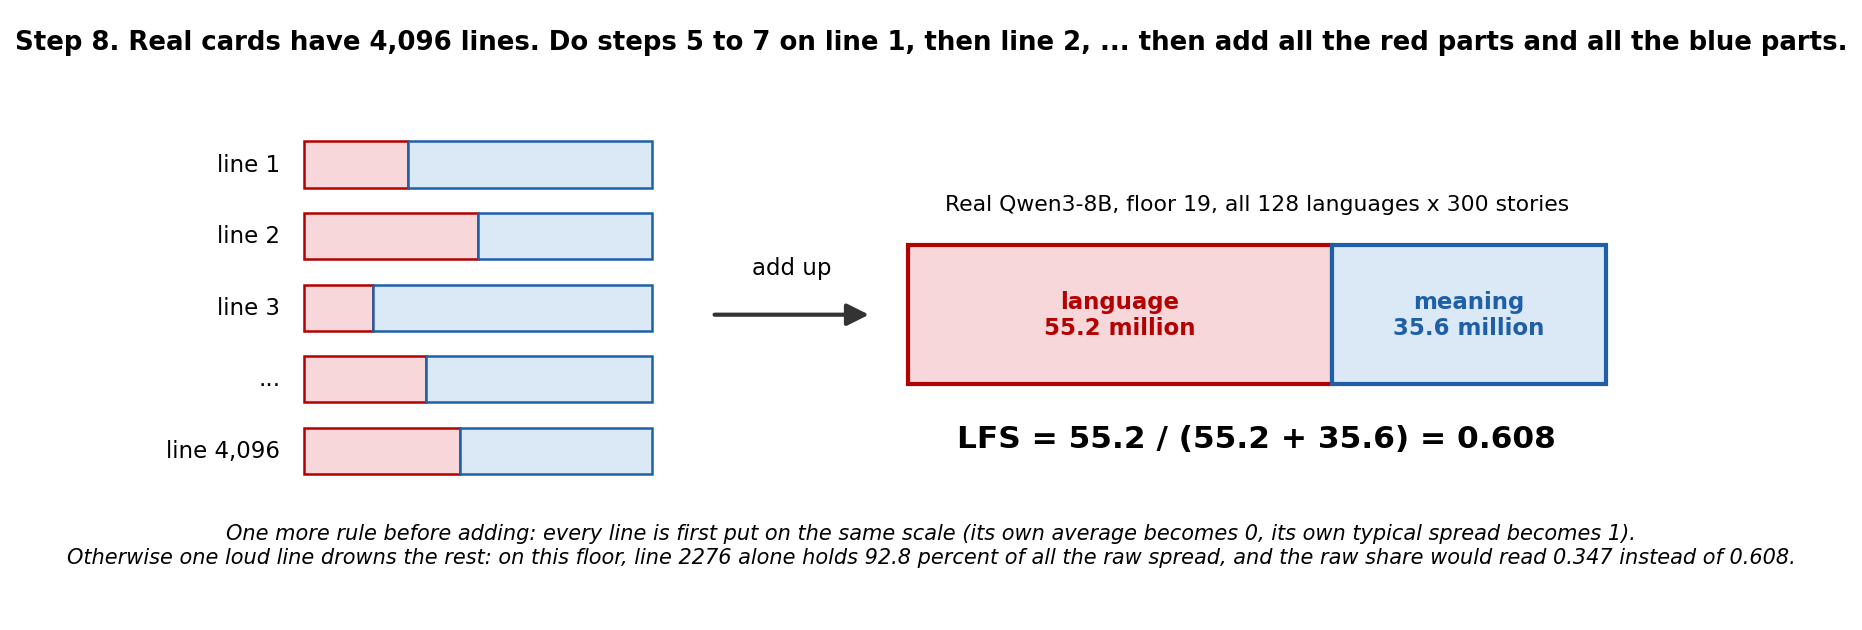
\includegraphics[width=0.98\linewidth]{figs/steps/s08_add_up_lines.png}\end{figure}
A real card has 4,096 lines. Do steps 5 to 7 on each line and add up all the red parts and all the blue parts. On floor 19 of Qwen3-8B the red total is 55.2 million and the blue total is 35.6 million, so LFS is 0.608. One rule first: put every line on the same scale before adding, or one loud line drowns the rest. On this floor a single line, number 2276, holds 92.8 percent of the raw spread by itself, and without the rule the share would wrongly read 0.347.

\subsection*{Step 9. The curve}
\begin{figure}[H]\centering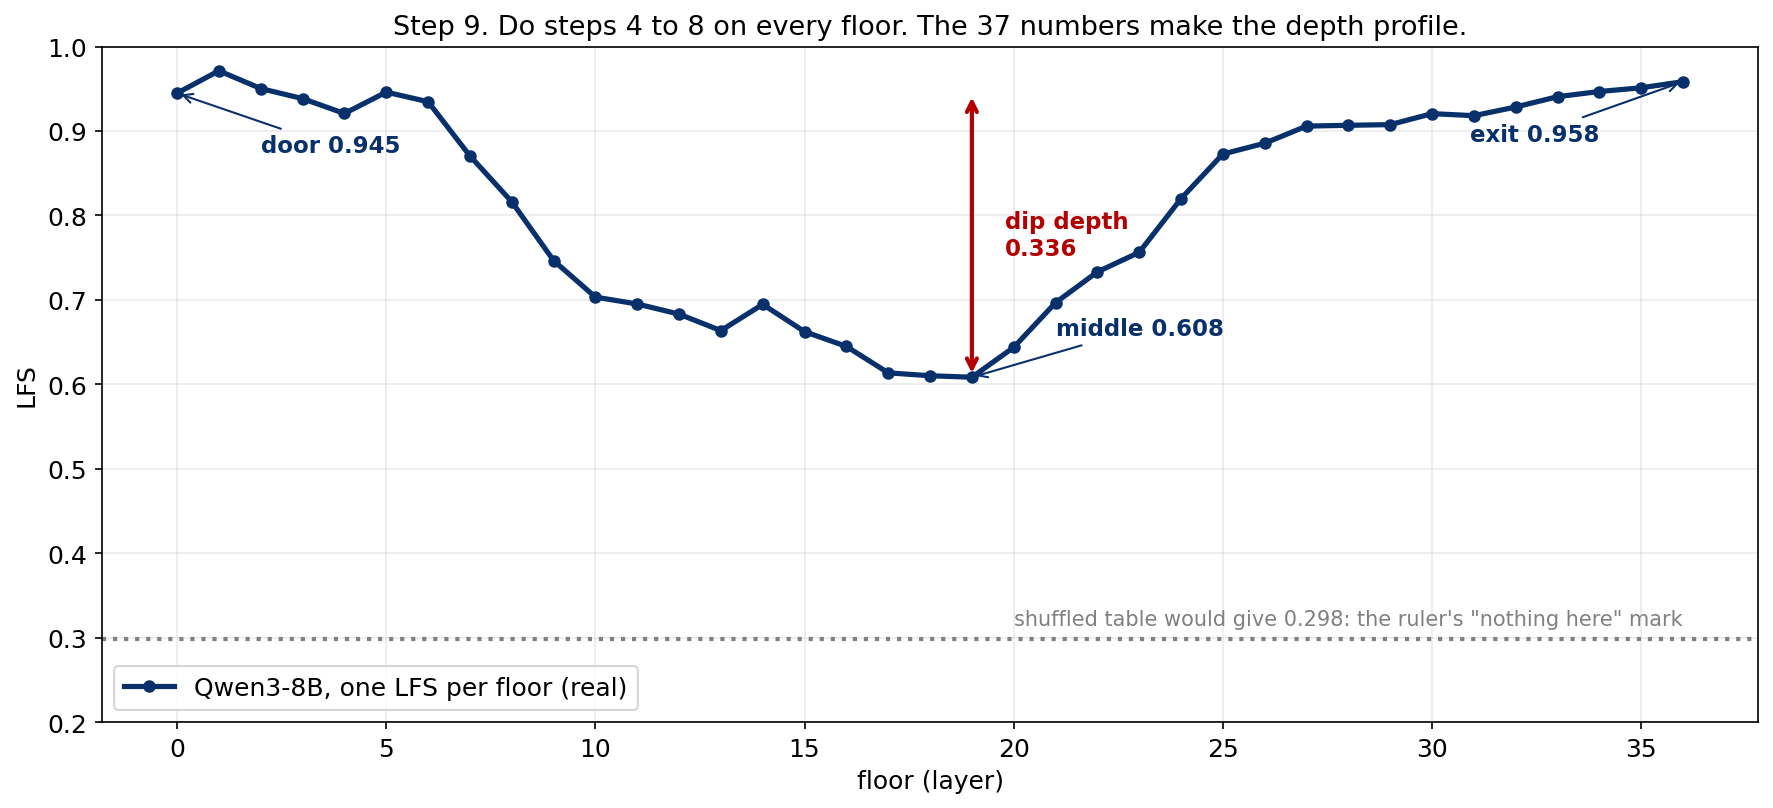
\includegraphics[width=0.95\linewidth]{figs/steps/s09_curve_real.png}\end{figure}
Do it on every floor and you get 37 numbers: the depth profile. Door 0.945, middle 0.608, exit 0.958. The drop from door to middle is the dip depth, 0.336. The dotted line at 0.298 is what a shuffled, meaningless table would give, so it is the ruler's ``nothing here'' mark.

\subsection*{Step 10. Reading the curve}
\begin{figure}[H]\centering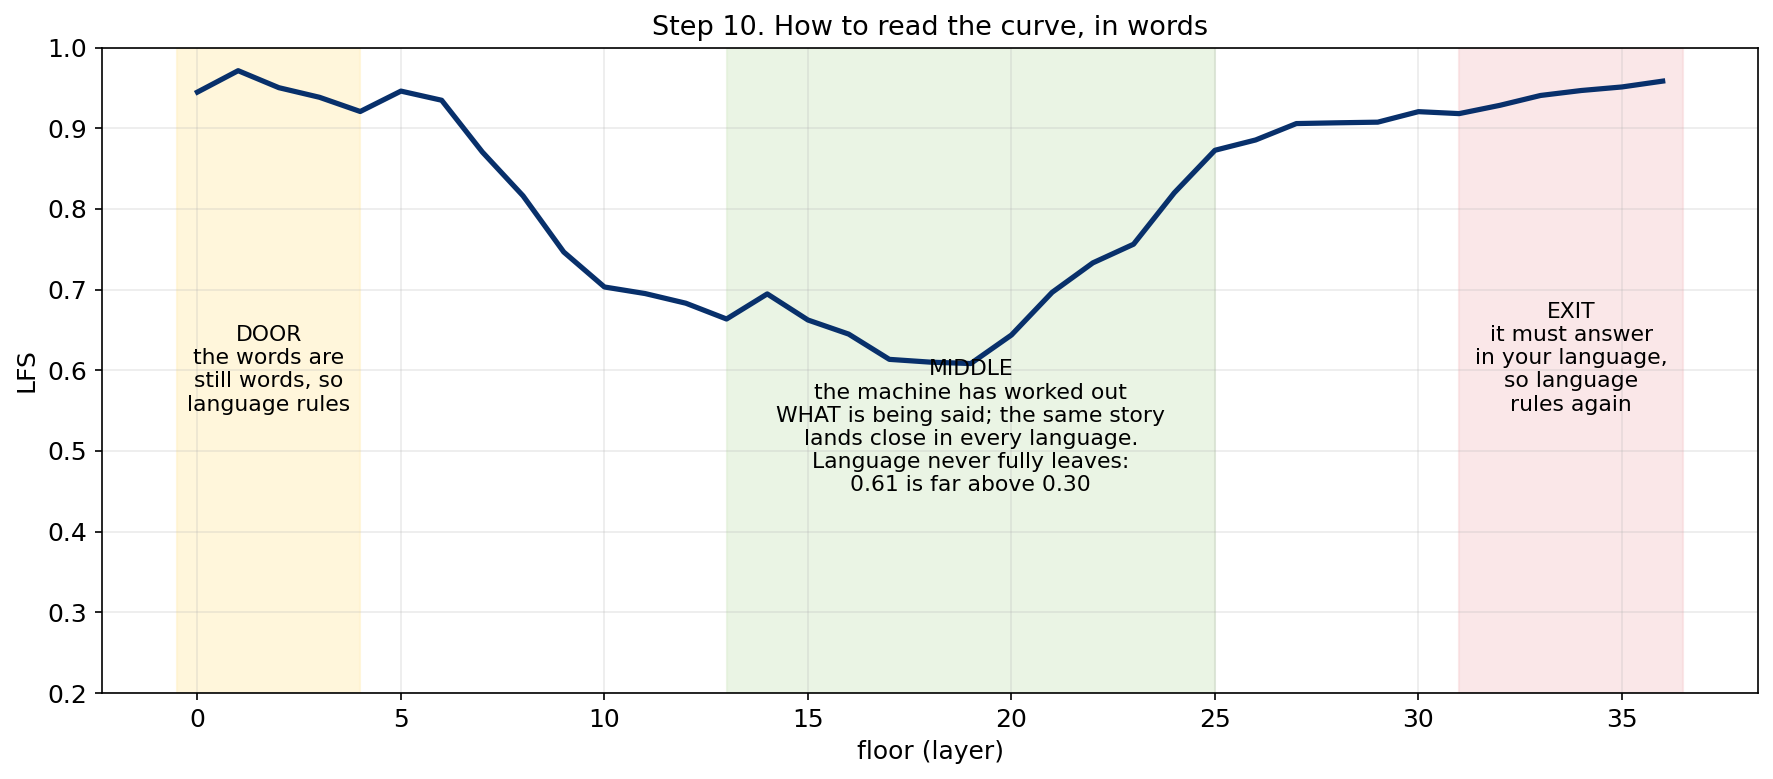
\includegraphics[width=0.95\linewidth]{figs/steps/s10_reading_curve.png}\end{figure}
At the door the cards are still mostly the words, so language rules. In the middle the machine has worked out what is being said, so the same story lands close in every language and language matters least, though it never leaves. At the exit the machine must answer in your language, so language rules again.

\subsection*{Step 11. What the ruler cannot do}
\begin{figure}[H]\centering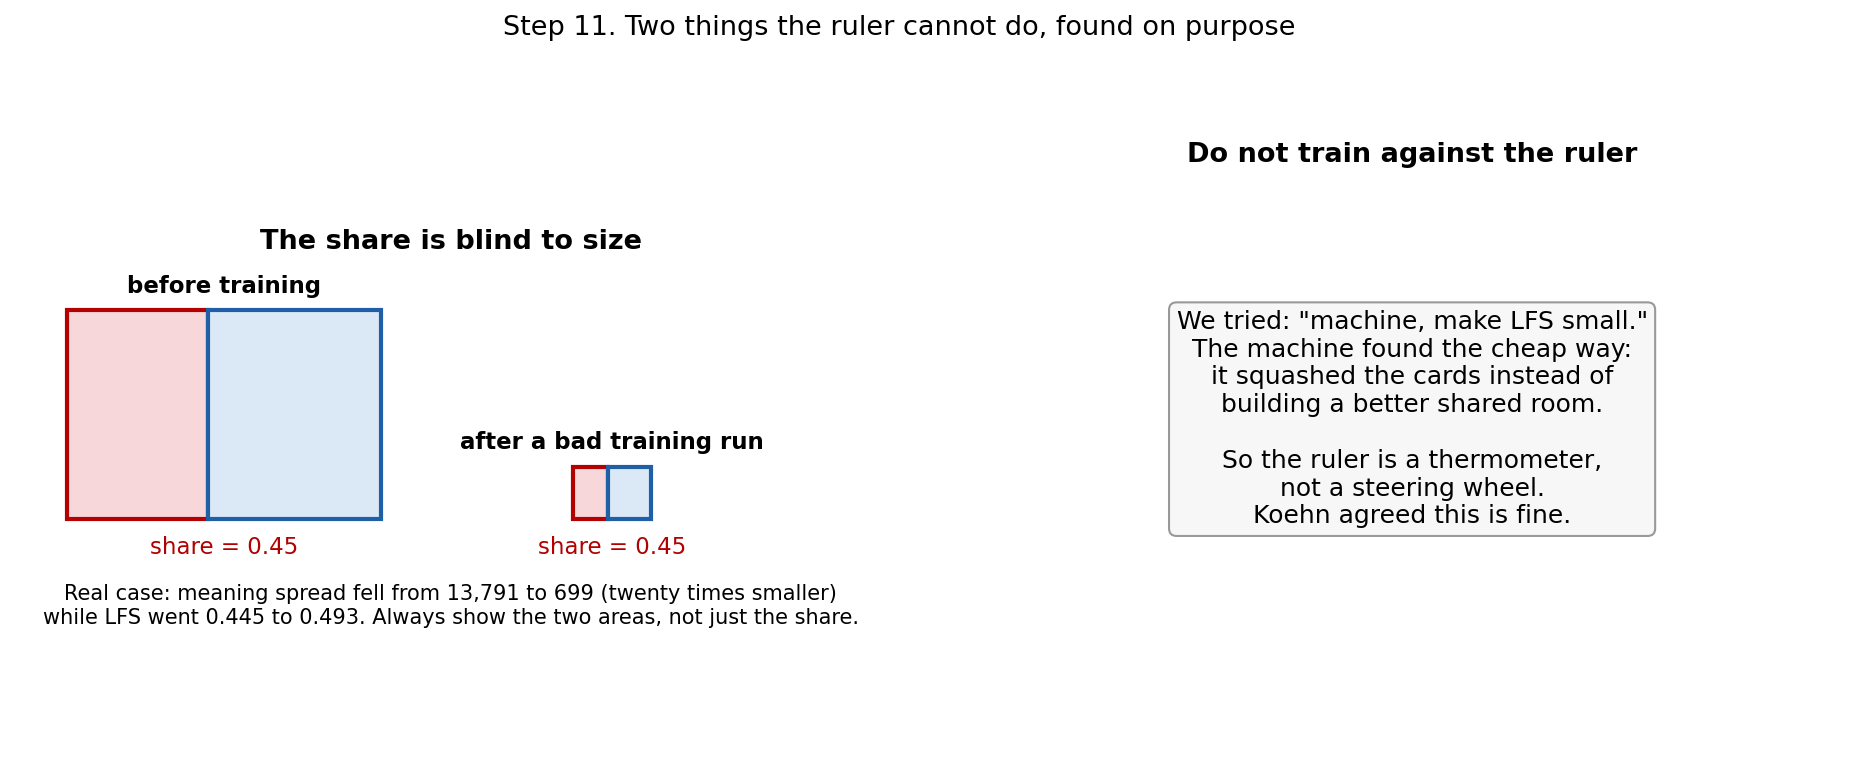
\includegraphics[width=0.98\linewidth]{figs/steps/s11_cannot.png}\end{figure}
A share is blind to size: a big bar and a tiny bar can both be 45 percent red. In one training run the meaning spread shrank twenty times while LFS barely moved, so we always show the two areas beside the share. And when we told a machine ``make LFS small,'' it squashed the cards instead of building a better shared room. So the ruler is a thermometer, not a steering wheel. Professor Koehn agreed that Aim 2 does not need the ruler as a training target.

\subsection*{Step 12. Back to the proposal}
\begin{figure}[H]\centering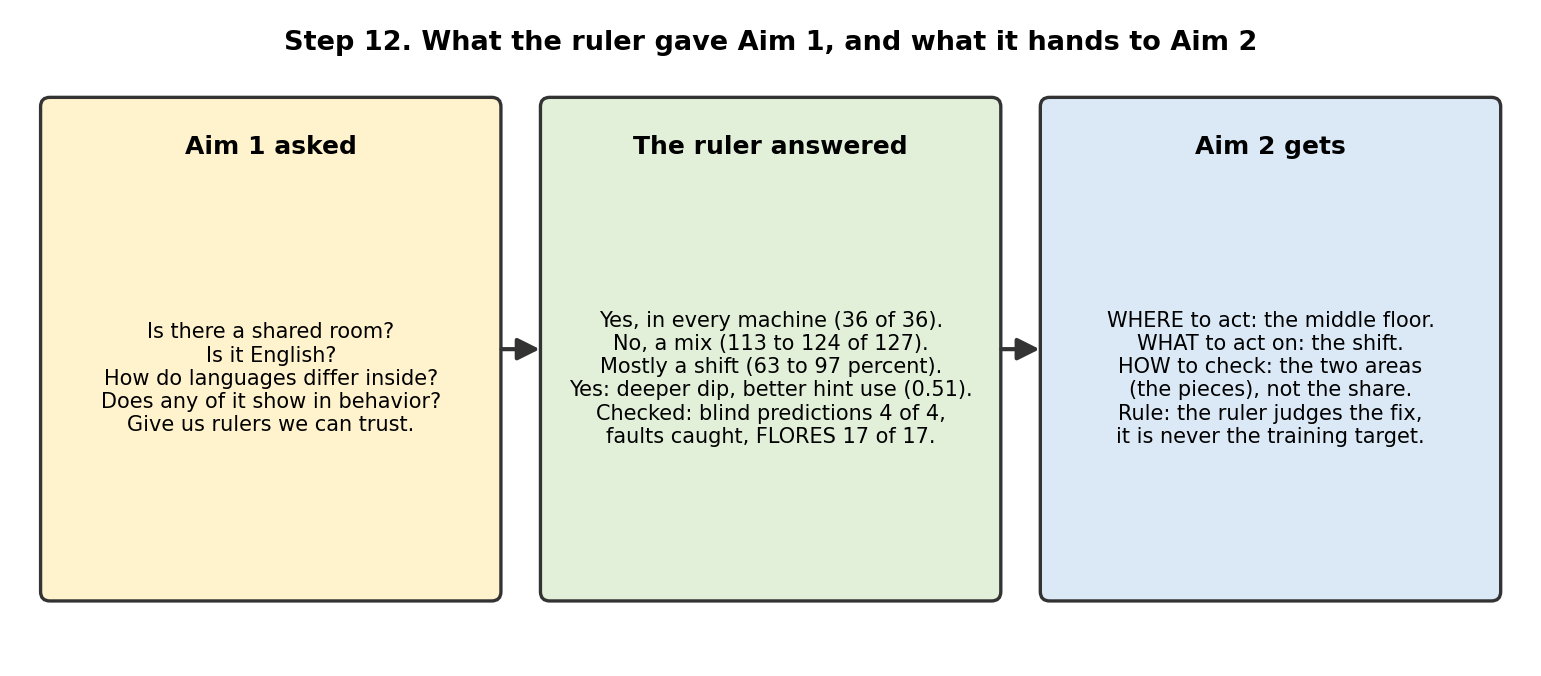
\includegraphics[width=0.98\linewidth]{figs/steps/s12_aims.png}\end{figure}
Aim 1 asked five questions; each got a measure and an answer. Aim 2 gets three things from that: where to act (the middle floors), what to act on (the shift), and how to check the fix (the two areas, not the share).

\section*{Part D. Say it back}
\begin{framed}
``The professors asked how strong the language part of a representation is, and whether the middle of the machine is one shared room or an English room with copies. I built a ruler, LFS, that says floor by floor how much of the layout is language and how much is meaning. Every machine has a shared room in the middle. It is not English. What is left of language there is mostly a shift. Machines with a deeper middle use hints from other languages more. The ruler is checked against a second dataset, blind predictions, and injected faults, and it is for looking, not for training.''
\end{framed}

Grown-up words for the same things: a card is a hidden state; a floor is a layer; averaging the pieces is mean pooling; the table is the language-by-sentence grid; the red and blue areas are the language and concept sums of squares; the share is the Language-Factor Share; the ``nothing here'' mark is the null, 0.298; the shared room is the shared representation; the shift is an additive offset; the hint test is cross-lingual content transfer; the hub test asks whether the shared factor is English; putting lines on the same scale is standardization.

\end{document}
